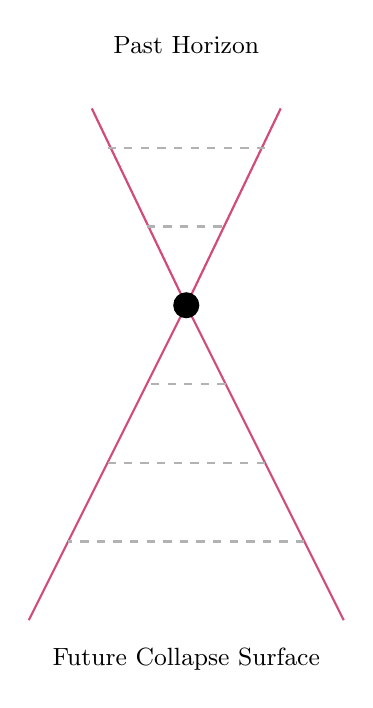
\begin{tikzpicture}[
    cone/.style={draw=purple!70, thick},
    slice/.style={draw=gray!60, dashed, thick}
]

\draw[cone] (0,0) -- (-2,-4);
\draw[cone] (0,0) -- (2,-4);
\draw[cone] (0,0) -- (-1.2,2.5);
\draw[cone] (0,0) -- (1.2,2.5);

\foreach \y in {-3,-2,-1,1,2}{
  \draw[slice] (-2*\y/4,\y) -- (2*\y/4,\y);
}

\node at (0,0) [circle,fill=black,minimum size=5pt]{};

\node at (0,3.3) {\small Past Horizon};
\node at (0,-4.5) {\small Future Collapse Surface};

\end{tikzpicture}